\chapter{Lecture 1: New Revolutions in Particle Physics: Standard Model}

These notes follow Leonard Susskind's first lecture in \emph{Particle Physics 2: Standard Model}, with curation by LazyingArt LLC. The lecture begins by refusing, for a few minutes more, to do the thing it has promised to do, namely to list the particles. That delay is deliberate. Before we start cataloguing the players, we want the conceptual triangle to be complete: particles, the fields of which they are quanta, and the forces that arise when those quanta can be exchanged. The chapter therefore opens with force, first in classical field language, then in quantum exchange language, and only after that turns to the particle table.

\section{Particles, Fields, and the Missing Third Leg}

Up to this point the course has already built a substantial framework. We have fields, their quanta, wave equations, action principles, spin, and the sharp distinction between bosons and fermions. We also know that interaction terms in a Lagrangian codify elementary processes: particles come in, particles go out, and the field operators tell us which transitions are allowed.

But there is still a missing leg. The lecture insists on the following correspondence:
\begin{itemize}
\item particles,
\item fields of which those particles are quanta,
\item forces associated with exchange processes involving those same quanta.
\end{itemize}

There is also a deliberate warning here. The distinction between elementary and composite particles is real, but slippery, and we are not going to settle it at the outset. For the moment we imagine that there are fundamental fields and that their quanta are the elementary particles. The point of the evening is then to understand why the story does not stop there: for each such field there is also, in a suitable sense, a force.

The lecture's guiding theme can be stated in one sentence: if fields and particles are two languages for the same physics, then force must admit both a field-language description and a particle-language description.

\section{Force from Field Energy in Classical Electrodynamics}

Susskind begins in the classical language because the structure is especially transparent there. Put two charges into space. We may of course memorize the Coulomb law, but the lecture asks a better question: what do the charges \emph{do} to space?

They create electric fields. If the first charge produces a field \(\mathbf{E}_1\) and the second a field \(\mathbf{E}_2\), then the total field is
\begin{equation}
\mathbf{E}=\mathbf{E}_1+\mathbf{E}_2.
\end{equation}
The transcript in this part is noisy about overall factors and about a temporary charge-rescaled notation, so we keep only the stable mathematical backbone. The field energy is obtained schematically by squaring the field and integrating over space:
\begin{equation}
U_{\text{field}}\propto \int d^3x\,\mathbf{E}^2.
\end{equation}
Substituting the sum of the two fields gives
\begin{align}
U_{\text{field}}
&\propto \int d^3x\,(\mathbf{E}_1+\mathbf{E}_2)^2 \\
&\propto \int d^3x\,\bigl(\mathbf{E}_1^2+\mathbf{E}_2^2+2\,\mathbf{E}_1\!\cdot\!\mathbf{E}_2\bigr).
\end{align}

Now the lecture slows down and interprets the three terms one by one.

The first two terms are self-energies. Each belongs to one isolated charge. Each is position-independent. Each is already part of the mass-energy budget of that particle. In modern language one might say that these are folded into the renormalized masses. The lecture does not pursue that formalism here; it simply says: forget those terms, they are already there.

The third term is the interesting one. It is not the energy of either charge taken alone. It depends on the overlap of the two fields, and therefore on the separation between the charges. If the charges are taken infinitely far apart, the overlap becomes negligible and the cross-term tends to zero. If the charges are brought closer together, the overlap grows, and so does this interaction contribution. Thus one is naturally led to define, again schematically,
\begin{equation}
U_{\text{int}}(r)\propto \int d^3x\,\mathbf{E}_1\!\cdot\!\mathbf{E}_2.
\end{equation}
The force is then read from the separation dependence of this energy:
\begin{equation}
F(r)=-\frac{dU_{\text{int}}}{dr}.
\end{equation}
If one works the integral out in the Coulomb case, one recovers the familiar law
\begin{equation}
F_{\text{Coulomb}}(r)\propto \frac{q_1 q_2}{r^2}.
\end{equation}

This is a pure field-theoretic picture. The force law is not imported from outside. It appears because the presence of both charges changes the field energy in a way that depends on the distance between them.

\section{Molecular Exchange: Two Protons and One Electron}

The lecture now makes a sharp turn. Before rephrasing electrodynamics in particle language, Susskind chooses a system in which the exchange picture is easier to see: two protons and a single electron.

If one proton is present and the other is taken very far away, the electron has the familiar hydrogenic ground state. The board first records this as a single localized hump. The visual point is not quantitative accuracy but localization.

\begin{figure}[h]
\centering

\includegraphics[width=0.72\textwidth]{lecture_01_figure_02.png}

\medskip

\begin{tikzpicture}[scale=0.95]
\draw (-0.2,0) -- (6.4,0);
\fill (1.3,0) circle (2pt);
\draw[smooth] plot coordinates {(0.1,0.15) (0.8,1.15) (1.5,1.75) (2.2,1.1) (3.0,0.35) (3.8,0.12)};
\node at (1.3,-0.35) {$p$};
\node at (2.7,1.55) {$\psi_1(x)$};
\end{tikzpicture}
\caption{Single localized ground-state profile near one proton. The board image is kept as evidence, while the TikZ sketch gives a cleaned schematic interpretation.}
\end{figure}

Now place a second proton at finite but large separation. By symmetry there is another localized state of the same energy, centered near the second proton. The board then develops into the left-right two-center picture.

\begin{figure}[h]
\centering

\includegraphics[width=0.78\textwidth]{lecture_01_figure_03.png}

\medskip

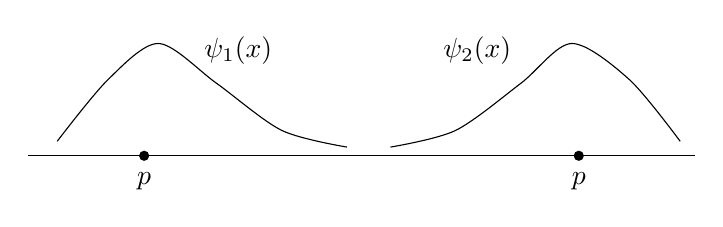
\begin{tikzpicture}[scale=0.92]
\draw (-0.2,0) -- (9.0,0);
\fill (1.4,0) circle (2pt);
\fill (7.4,0) circle (2pt);
\draw[smooth] plot coordinates {(0.2,0.2) (0.9,1.05) (1.6,1.55) (2.4,1.0) (3.3,0.35) (4.2,0.12)};
\draw[smooth] plot coordinates {(4.8,0.12) (5.7,0.35) (6.6,1.0) (7.3,1.55) (8.1,1.05) (8.8,0.2)};
\node at (1.4,-0.35) {$p$};
\node at (7.4,-0.35) {$p$};
\node at (2.7,1.45) {$\psi_1(x)$};
\node at (6.0,1.45) {$\psi_2(x)$};
\end{tikzpicture}
\caption{Two localized one-center wave functions. The lecture then turns this two-state picture into an equilibrium superposition.}
\end{figure}

At infinite separation these two states are degenerate. The electron can be localized near the left proton or near the right proton, and the energy is the same.

\subsection{Question \& Answer}

\paragraph{Question.} Why is the two-proton system not exactly degenerate once the separation is finite?

\paragraph{Answer.} Because new processes become possible. If the protons are not infinitely far apart, the electron can tunnel from one center to the other. In the lecture this is first described qualitatively, but the simplest mathematical reconstruction is a two-state model. Let \(|L\rangle\) and \(|R\rangle\) denote the two localized states. Then the finite-separation Hamiltonian contains off-diagonal mixing:
\begin{align}
H|L\rangle &= E_0 |L\rangle - t |R\rangle,\\
H|R\rangle &= E_0 |R\rangle - t |L\rangle,
\end{align}
with \(t>0\) a tunneling matrix element.

The energy eigenstates are therefore not \(|L\rangle\) and \(|R\rangle\) themselves but the symmetric and antisymmetric combinations
\begin{align}
|+\rangle &= \frac{|L\rangle+|R\rangle}{\sqrt2}, &
E_+ &= E_0-t,\\
|-\rangle &= \frac{|L\rangle-|R\rangle}{\sqrt2}, &
E_- &= E_0+t.
\end{align}
In the language of wave functions, the lower state is approximately
\begin{equation}
\psi_+(x)\approx \frac{\psi_1(x)+\psi_2(x)}{\sqrt2}.
\end{equation}
This is precisely the lecture's point: the equilibrium wave function is the symmetric superposition, though the exact wave function is \emph{not} exactly the naive sum. In the overlap region it is slightly corrected. That slight correction is enough to matter energetically.

The lecture is also careful to say what one should not do. One should not stand in the middle and try to watch a literal particle trajectory from one well to the other. The exchange picture is a way of describing the quantum state, not a surveillance video of the electron.

\section{From Lowered Energy to an Effective Force}

Once the equilibrium state is in place, the lecture turns from shape to energy. If the two protons are very far apart, the electron energy is just the ordinary hydrogenic ground-state energy. As the protons are brought closer, the possibility of tunneling and superposition lowers the energy slightly. That lowered amount depends on the separation \(r\). Hence one may think of it as an effective potential \(V(r)\) between the two protons.

The board then adds a second layer: below the wave-function sketches appears a qualitative energy curve. The frame does not fix whether the vertical quantity should be called \(E(r)\) or \(V(r)\), so we use \(V(r)\) consistently in the text while keeping the graph qualitative.

\begin{figure}[h]
\centering

\includegraphics[width=0.78\textwidth]{lecture_01_figure_04.png}

\medskip

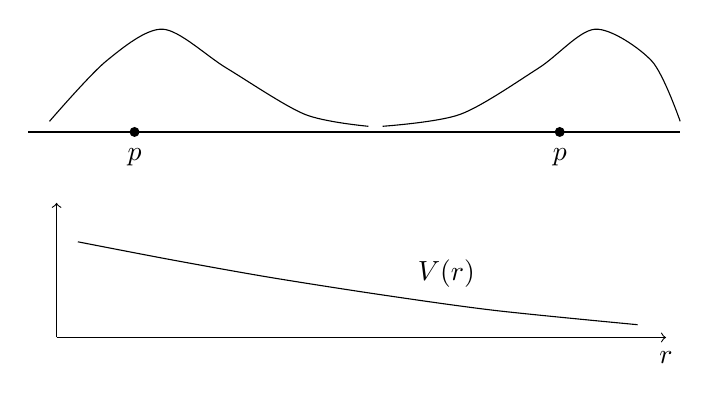
\begin{tikzpicture}[scale=0.9]
\draw (-0.2,3.0) -- (9.0,3.0);
\fill (1.3,3.0) circle (2pt);
\fill (7.3,3.0) circle (2pt);
\draw[smooth] plot coordinates {(0.1,3.15) (0.9,4.0) (1.7,4.45) (2.6,3.9) (3.7,3.25) (4.6,3.08)};
\draw[smooth] plot coordinates {(4.8,3.08) (5.9,3.25) (7.0,3.9) (7.8,4.45) (8.6,4.0) (9.0,3.15)};
\node at (1.3,2.65) {$p$};
\node at (7.3,2.65) {$p$};

\draw[->] (0.2,0.1) -- (0.2,2.0);
\draw[->] (0.2,0.1) -- (8.8,0.1);
\draw[smooth] plot coordinates {(0.5,1.45) (1.8,1.2) (3.2,0.95) (4.8,0.7) (6.4,0.48) (8.4,0.28)};
\node at (5.7,1.0) {$V(r)$};
\node at (8.8,-0.18) {$r$};
\end{tikzpicture}
\caption{Upper board: two-center wave functions. Lower board: a qualitative potential-energy curve versus proton separation. The label \(V(r)\) is a cleaned choice; the board itself leaves the axes effectively unlabeled.}
\end{figure}

The force is now read off exactly as it was in the classical field example:
\begin{equation}
F(r)=-\frac{dV}{dr}.
\end{equation}
If \(V(r)\) decreases as the protons move closer over some range, the force points inward, toward smaller \(r\). That is the attractive piece of the covalent bond.

\paragraph{What the picture is not.} The lecture spends time ruling out several tempting but wrong simplifications.
\begin{itemize}
\item The effect is not merely a screening of the proton charges.
\item It is not a literal third independent force acting in addition to the known interactions.
\item It is not best described as ordinary two-particle entanglement; the more relevant statement is that there are off-diagonal matrix elements in the Hamiltonian linking the two localized states.
\item The worldline picture is only schematic. Watching the electron in the middle would destroy the tunneling phenomenon.
\end{itemize}

Even in the one-electron system there is still Coulomb repulsion between the protons, so attraction does not automatically imply binding at all distances. The exchange-induced attraction is comparatively short-range, whereas the electrostatic repulsion falls off more slowly. This is why the lecture repeatedly speaks of a competition of effects rather than a miracle cancellation.

Still, the exchange language is pedagogically useful, and the lecture reconstructs it pictorially.

\begin{figure}[h]
\centering
\begin{tikzpicture}[scale=1.0]
\draw (0,0) -- (0,4.4);
\draw (4.8,0) -- (4.8,4.4);
\draw (0,0.9) .. controls (1.6,1.7) and (3.2,1.7) .. (4.8,2.5);
\draw (4.8,2.9) .. controls (3.2,2.1) and (1.6,2.1) .. (0,3.9);
\node at (0,-0.35) {proton};
\node at (4.8,-0.35) {proton};
\node at (2.35,1.55) {$e^-$};
\node at (2.35,2.55) {$e^-$};
\end{tikzpicture}
\caption{Transcript-backed schematic of electron exchange between two proton worldlines. This is an explanatory reconstruction of the lecture's picture, not a literal board transcription.}
\end{figure}

\section{Photon, Electron, and Quantum Electrodynamics}

Only after the molecular detour does the lecture return to electrodynamics and ask the central question: can the Coulomb force be told in the same exchange language? The answer is yes. A charged particle interacts with the electromagnetic field, and the quanta of that field are photons. In classical language we solve for the electric field. In quantum field theory we instead think in terms of emission and absorption of photons.

A physical charged particle is therefore not just a bare charge with no surroundings. It is a quantum superposition of states with zero photons, one photon, two photons, and so on, emitted and reabsorbed in equilibrium. If a second charged particle is nearby, then a photon emitted by one can be absorbed by the other. That process creates a separation-dependent contribution to the energy, and that energy is the Coulomb interaction in particle language.

The lecture's moral is by now clear: classical overlap energy and quantum exchange energy are not two unrelated stories. They are two descriptions of the same underlying phenomenon.

The board now switches into catalog mode. The visible photon row is worth keeping because it marks the change of pace from conceptual prelude to inventory.

\begin{figure}[h]
\centering

\includegraphics[width=0.7\textwidth]{lecture_01_figure_05.png}
\caption{The beginning of the particle table. The board visibly shows the photon row, the symbol \(\gamma\), and the field notation \(A\).}
\end{figure}

The lecture explicitly says that the photon's field is called \(A\). In modern covariant notation one often writes \(A_\mu\), but the board itself only visibly shows \(A\), so we keep that notation first and sharpen it only in prose when necessary.

\begin{table}[h]
\centering
\begin{tabular}{lllllll}
Name & Symbol & Field & Type & \(Q\) & \(B\) & Mass \\
Photon & \(\gamma\) & \(A\) & boson & \(0\) & \(0\) & \(0\) \\
Electron/positron & \(e^\pm\) & \(\psi_e\) & fermion & \(\mp 1\) & \(0\) & \(0.51\,\mathrm{MeV}\)
\end{tabular}
\caption{A cleaned summary of the first two entries discussed in the lecture. The board crop does not fully expose the heading above \(A\), but the lecture makes clear that \(A\) is the photon's field.}
\end{table}

The elementary QED process is the familiar three-legged vertex: one electron in, one electron out, one photon attached. At the level of the lecture it is enough to write the corresponding interaction schematically as
\begin{equation}
\mathcal{L}_{\mathrm{int}}\sim e\,\psi_e^\dagger \psi_e A,
\end{equation}
with the understanding that this is a cleaned schematic statement, not the full covariant textbook formula. The point being emphasized is simpler: the coupling constant is the electric charge \(e\), so the amplitude for photon emission is proportional to \(e\), and the probability is correspondingly proportional to \(e^2\).

The exchange picture of the Coulomb force can then be sketched directly.

\begin{figure}[h]
\centering
\begin{tikzpicture}[scale=1.0]
\draw (0,0) -- (0,4.0);
\draw (4.8,0) -- (4.8,4.0);
\draw (0,2.0) -- (4.8,2.0);
\node at (0,-0.35) {$e^-$};
\node at (4.8,-0.35) {$e^-$};
\node at (2.4,2.3) {$\gamma$};
\end{tikzpicture}
\caption{Transcript-backed schematic of photon exchange. In the lecture this is the quantum-field-theoretic retelling of the Coulomb interaction.}
\end{figure}

At this point the missing third leg has been supplied. We may now proceed to the particle list without feeling that we have merely memorized names.

\section{Quarks, Baryon Number, and Families}

The lecture next turns from the familiar photon and electron to the objects that organize modern hadronic physics: quarks. Instead of taking protons and neutrons as basic, we now regard them as composites of more elementary constituents.

There are six quark flavors:
\begin{equation}
u,\ d,\ s,\ c,\ b,\ t.
\end{equation}
They are all fermions. Their electric charges come in a repeated pattern:
\begin{equation}
Q(u)=Q(c)=Q(t)=+\frac23,
\qquad
Q(d)=Q(s)=Q(b)=-\frac13.
\end{equation}
The lecture stresses the pattern of replication. The pair \((d,u)\) is echoed by \((s,c)\), which is echoed again by \((b,t)\). Yet the masses do not repeat in any simple way:
\begin{align}
m_u &\sim 5\,\mathrm{MeV}, &
m_d &\sim 10\,\mathrm{MeV},\\
m_s &\sim 100\,\mathrm{MeV}, &
m_c &\sim 10^3\,\mathrm{MeV},\\
m_b &\sim 5\,\mathrm{GeV}, &
m_t &\sim 170\,\mathrm{GeV}.
\end{align}
In one sense the six quarks are strikingly similar; in another sense their masses wander wildly over the map. The lecture insists that this is not understood in any deep way. One may infer a mass, as was historically done for the top quark, from its effects inside other processes, but that is not the same thing as explaining why the mass has that value.

\subsection{Question \& Answer}

\paragraph{Question.} Why does a quark carry baryon number \(1/3\), and can baryon number be violated?

\paragraph{Answer.} Baryon number is first introduced as a bookkeeping device for protons and neutrons. By convention
\begin{equation}
B(p)=1, \qquad B(n)=1.
\end{equation}
If a proton is later understood to be made of three quarks, then consistency forces
\begin{equation}
B(q)=\frac13,
\qquad
B(\bar q)=-\frac13.
\end{equation}
So the factor \(1/3\) is not mysterious at the level of bookkeeping; it is inherited from the earlier convention that a proton carries unit baryon number.

The deeper question is whether baryon number is exact. Empirically it is extraordinarily well conserved, but the lecture is careful not to elevate that empirical fact into a theorem. A hypothetical decay such as
\begin{equation}
p\to e^+ + \gamma
\end{equation}
would conserve electric charge while violating baryon number. No such process has been observed, and the proton lifetime is constrained to be at least of order \(10^{33}\) to \(10^{34}\) years, but the lecture leaves the door open: baryon conservation may be approximate rather than absolute.

There is also a practical warning. Quarks are not observed as isolated free particles. One can certainly detect evidence for them, but not an isolated quark calmly separated from everything else and displayed on a table.

\section{From Quarks to Hadrons and Mesons}

Once the quark charges are known, familiar hadrons can be rebuilt in the new language. The neutron and proton are the first examples:
\begin{equation}
n=ddu,
\qquad
p=uud.
\end{equation}
Their electric charges follow at once.

\paragraph{Worked example.}
\begin{align}
Q(n) &= Q(d)+Q(d)+Q(u)
= -\frac13-\frac13+\frac23
=0,\\
Q(p) &= Q(u)+Q(u)+Q(d)
= \frac23+\frac23-\frac13
=1.
\end{align}

If we ignore electromagnetism for a moment, the proton and neutron look almost identical. One is obtained from the other by interchanging \(u\) and \(d\). The lecture uses this near-symmetry to make a physical point. Since \(m_d>m_u\), the neutron, which contains more down quarks, should be slightly heavier. And indeed it is. Electromagnetic self-energy would by itself tend to make the charged proton heavier, but the \(d-u\) mass difference wins, so \(m_n>m_p\) by roughly \(1.3\) to \(1.4\,\mathrm{MeV}\).

\begin{remark}
The lecture also points out an important mismatch: the quark masses add to only a few MeV, while the proton mass is about \(940\,\mathrm{MeV}\). So most of the nucleon mass is not simply the sum of constituent quark masses. Susskind flags this as a problem of field energy and binding dynamics rather than resolving it here in detail.
\end{remark}

The same constituent logic produces strange baryons. Replace one down quark by a strange quark and the charge pattern is unchanged, because \(s\) and \(d\) carry the same electric charge:
\begin{equation}
uds,\qquad uss,\qquad uus.
\end{equation}
These strange baryons are heavier than the ordinary nucleons and hence unstable, but they are perfectly natural from the quark point of view.

Mesons now enter as quark-antiquark composites. Their baryon number is zero because
\begin{equation}
B(q\bar q)=\frac13-\frac13=0.
\end{equation}
Restrict first to \(u\) and \(d\). The natural flavor basis states are
\begin{equation}
|\bar u d\rangle,\qquad |u\bar d\rangle,\qquad |\bar u u\rangle,\qquad |\bar d d\rangle.
\end{equation}
The two charged states are straightforward:
\begin{equation}
|\pi^-\rangle = |\bar u d\rangle,
\qquad
|\pi^+\rangle = |u\bar d\rangle.
\end{equation}

\subsection{Question \& Answer}

\paragraph{Question.} Why are the neutral meson states written as superpositions rather than as separate \(\bar u u\) and \(\bar d d\) particles?

\paragraph{Answer.} Because the lecture is doing quantum mechanics, not classical bookkeeping. The neutral basis states \(|\bar u u\rangle\) and \(|\bar d d\rangle\) need not themselves be mass eigenstates. One is allowed, indeed compelled, to superpose them. The two orthogonal combinations are
\begin{align}
|\pi^0\rangle &\approx \frac{|\bar u u\rangle-|\bar d d\rangle}{\sqrt2},\\
|\eta\rangle &\approx \frac{|\bar u u\rangle+|\bar d d\rangle}{\sqrt2}.
\end{align}
At the level of this lecture these are the combinations that matter physically. The pion triplet \(\pi^+,\pi^0,\pi^-\) goes together because the three masses are close; in the idealized limit \(m_u=m_d\), they would be even more nearly identical. The orthogonal neutral combination is the \(\eta\), which is similar in many ways but noticeably heavier.

Numerically, the lecture quotes
\begin{equation}
m_\pi \approx 140\,\mathrm{MeV},
\qquad
m_\eta \approx 500\,\mathrm{MeV}.
\end{equation}
Why the \(\eta\) sits so much higher is acknowledged to be a more complicated story than the lecture wishes to tell in its first hour.

Finally, once the strange quark is included, one obtains the strange mesons or \(K\)-mesons by replacing a \(d\) or \(\bar d\) with an \(s\) or \(\bar s\). The relevant flavor combinations are
\begin{equation}
\bar u s,\qquad u\bar s,\qquad \bar d s,\qquad d\bar s.
\end{equation}
Two are charged and two are neutral. Counting all light \(u,d,s\) quarks and antiquarks gives
\begin{equation}
3\times 3 = 9
\end{equation}
light flavor combinations altogether. The lecture ends here deliberately. The particle zoo has only just begun, but the organizing language is now in place.

\section{Summary}

The lecture opens by postponing the particle list and closes by making that postponement worthwhile. First, force is reconstructed from the overlap energy of classical fields. Then the same logic is translated into exchange language by way of molecular binding: two centers, tunneling, superposition, lowered energy, effective attraction. Only after that bridge has been built does the lecture begin the inventory of particles.

The resulting picture is the real content of the chapter. A particle is the quantum of a field. The same particle, when exchanged, produces a force. Photons do this in electrodynamics; electrons do this in molecular binding. With that correspondence in hand, the first entries of the Standard Model table become more than names: \(\gamma\) and \(A\), \(e^\pm\) and \(\psi_e\), then quarks, baryon number, nucleons, strange baryons, and meson superpositions. The catalogue is still messy, as Susskind says repeatedly, but it is no longer a list without a story.